\documentclass[a4paper,12pt]{article}

\usepackage{geometry}
\usepackage{graphicx}
\usepackage{float}
\usepackage{booktabs}
\usepackage{longtable}
\usepackage{array}
\usepackage{amsmath}
\usepackage{amssymb}
\usepackage{xcolor}
\usepackage{listings}
\usepackage{hyperref}
\usepackage{caption}
\usepackage{subcaption}
\usepackage{tikz}
\usetikzlibrary{positioning}
\graphicspath{{figures/}}

\geometry{left=2.5cm,right=2.5cm,top=2.6cm,bottom=2.6cm}
\setlength{\parindent}{0pt}
\setlength{\parskip}{0.55em}
\linespread{1.15}

\hypersetup{
  colorlinks=true,
  linkcolor=black,
  urlcolor=blue,
  citecolor=black
}

\lstset{
  basicstyle=\ttfamily\small,
  keywordstyle=\color{blue!70!black},
  commentstyle=\color{green!40!black},
  stringstyle=\color{red!60!black},
  numbers=left,
  numberstyle=\tiny\color{gray},
  frame=single,
  breaklines=true,
  tabsize=4,
  showstringspaces=false,
  columns=fullflexible
}

\newcommand{\placeholderfigure}[2]{
  \begin{figure}[H]
    \centering
    \begin{tikzpicture}
      \draw[gray, thick, dashed] (0,0) rectangle (12,5.5);
      \node[align=center, text=gray!80!black] at (6,2.75)
      {#1\\[0.6em]\small Suggested file: \path{#2}};
    \end{tikzpicture}
    \caption{#1, to be added}
  \end{figure}
}

\newcommand{\maybeimage}[2]{
  \IfFileExists{#2}{
    \begin{figure}[H]
      \centering
      \includegraphics[width=0.88\textwidth]{#2}
      \caption{#1}
    \end{figure}
  }{
    \placeholderfigure{#1}{#2}
  }
}

\title{\textbf{Experimental Report on a Vision-Based Maze Drawing System Using a 5-DOF Robotic Arm}}
\author{Project: Maze Robotic Arm Drawing System}
\date{\today}

\begin{document}

\maketitle

\begin{abstract}
This experiment implements a complete robotic system that converts a camera image of a hand-drawn paper maze into an executable drawing trajectory for a 5-DOF robotic arm. The input is a white-paper maze drawn with black lines, where the start point is marked in red and the goal point is marked in blue. The system first reconstructs the paper maze through perspective correction and image binarization, then performs A* path planning on an occupancy grid, and finally maps the 2-D path into physical paper coordinates and joint-space commands. The real-arm execution is handled through a TCP client-server interface and a serial connection to the arm controller. The project demonstrates an integrated robotics workflow that combines computer vision, graph search, forward/inverse kinematics, simulation, and real hardware control.
\end{abstract}

\tableofcontents
\newpage

\section{Experiment Overview}

The goal of this project is to let a robotic arm draw the solution path of a maze from an ordinary camera photo. Since the photo may contain perspective distortion, uneven illumination, shadows, and background clutter, the system first reconstructs a clean top-down maze image. It then plans a collision-free path from the red start marker to the blue goal marker. The resulting 2-D path is converted into physical coordinates on the paper and then into five joint commands through inverse kinematics.

\begin{figure}[H]
  \centering
  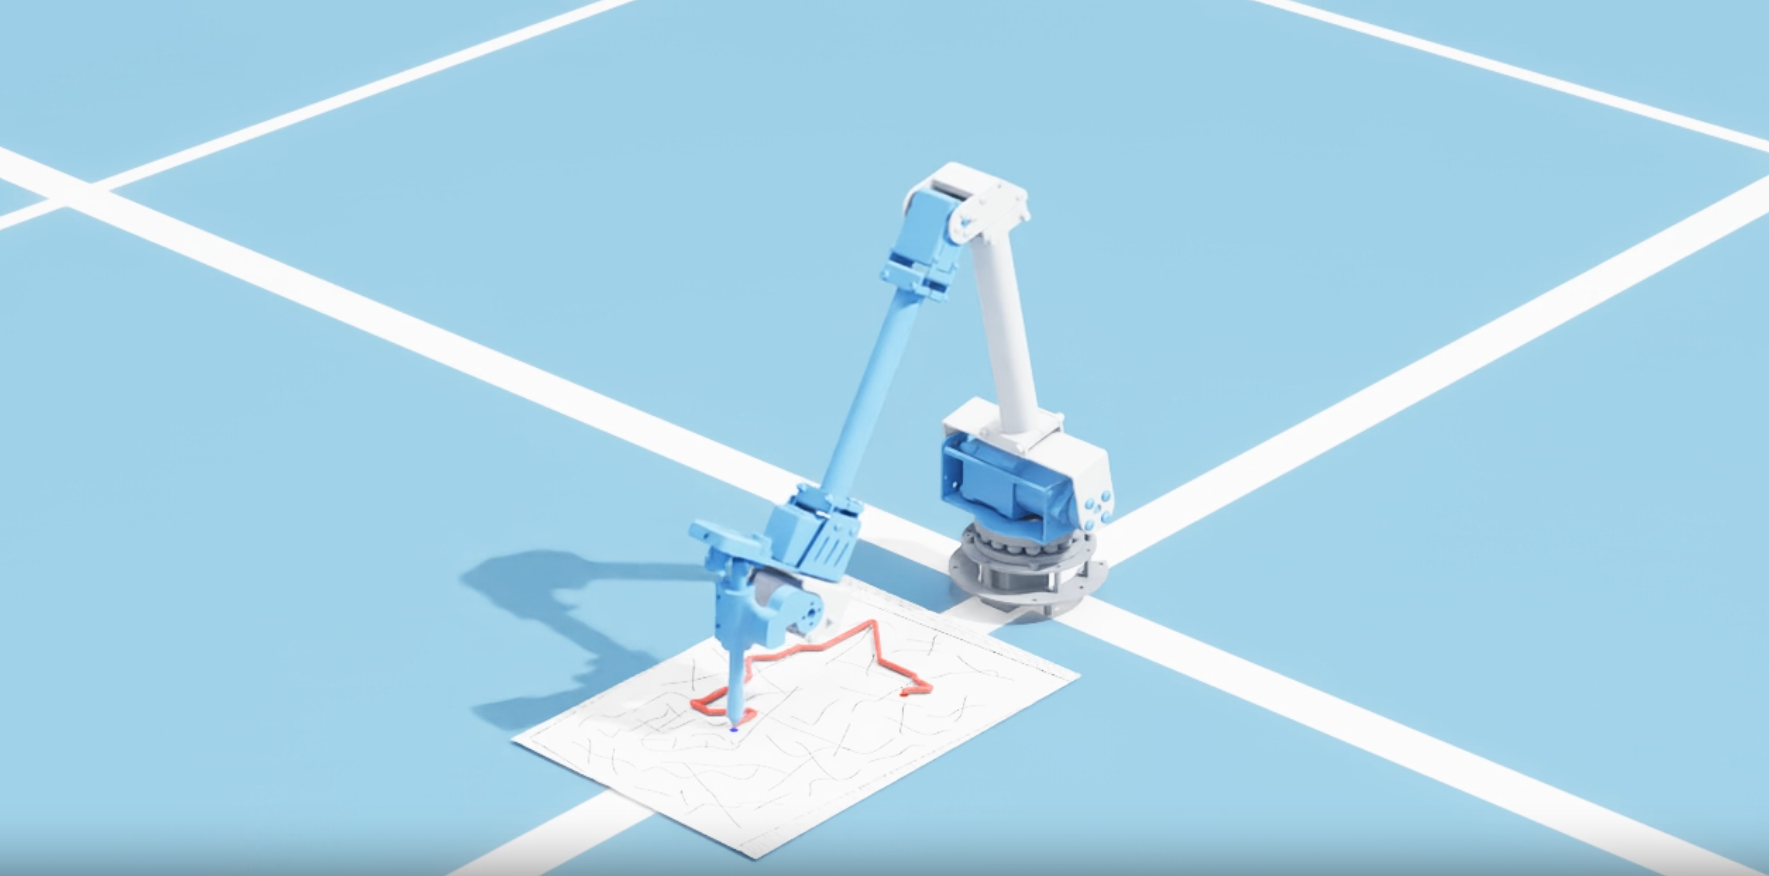
\includegraphics[width=0.88\textwidth]{overview.png}
  \caption{Overall project visualization}
\end{figure}

The system is divided into four major layers, as shown in Table \ref{tab:modules}.

\begin{table}[H]
  \centering
  \caption{Main system modules}
  \label{tab:modules}
  \begin{tabular}{p{3.2cm}p{6.2cm}p{4.8cm}}
    \toprule
    Module & Function & Main files \\
    \midrule
    Vision reconstruction & Recover a top-down binary maze image from a tilted photo & \texttt{maze\_planner/maze\_scanner.py} \\
    Path planning & Detect start/goal markers, build an occupancy grid, and run A* search & \texttt{maze\_planner/maze\_planner.py} \\
    Simulation & Import the 5-DOF robot into Isaac Sim and verify drawing behavior & \texttt{arm\_sim/draw\_maze.py} \\
    Real execution & Convert the path to joint commands and send them to the real arm & \texttt{arm\_real\_client/}, \texttt{arm\_real\_server/} \\
    \bottomrule
  \end{tabular}
\end{table}

\section{Hardware and Software Platform}

\subsection{Hardware Platform}

The experiment uses a 5-DOF desktop robotic arm. The original gripper is replaced by a pen holder so that the robot end-effector can draw on a sheet of paper. The arm communicates with a Windows lower-level host through USB serial and requires a separate 12 V power supply.

\maybeimage{Real robotic arm setup}{figures/real_setup.jpg}
\maybeimage{Close-up view of the pen mount}{figures/pen_mount.jpg}

The URDF model of the robot is stored in \texttt{urdf/five\_dof\_arm.urdf}, and the corresponding STL meshes are stored in \texttt{urdf/meshes/}. Figure \ref{fig:zero_pose} and Figure \ref{fig:reachable} show the simulated zero pose and reachable workspace.

\begin{figure}[H]
  \centering
  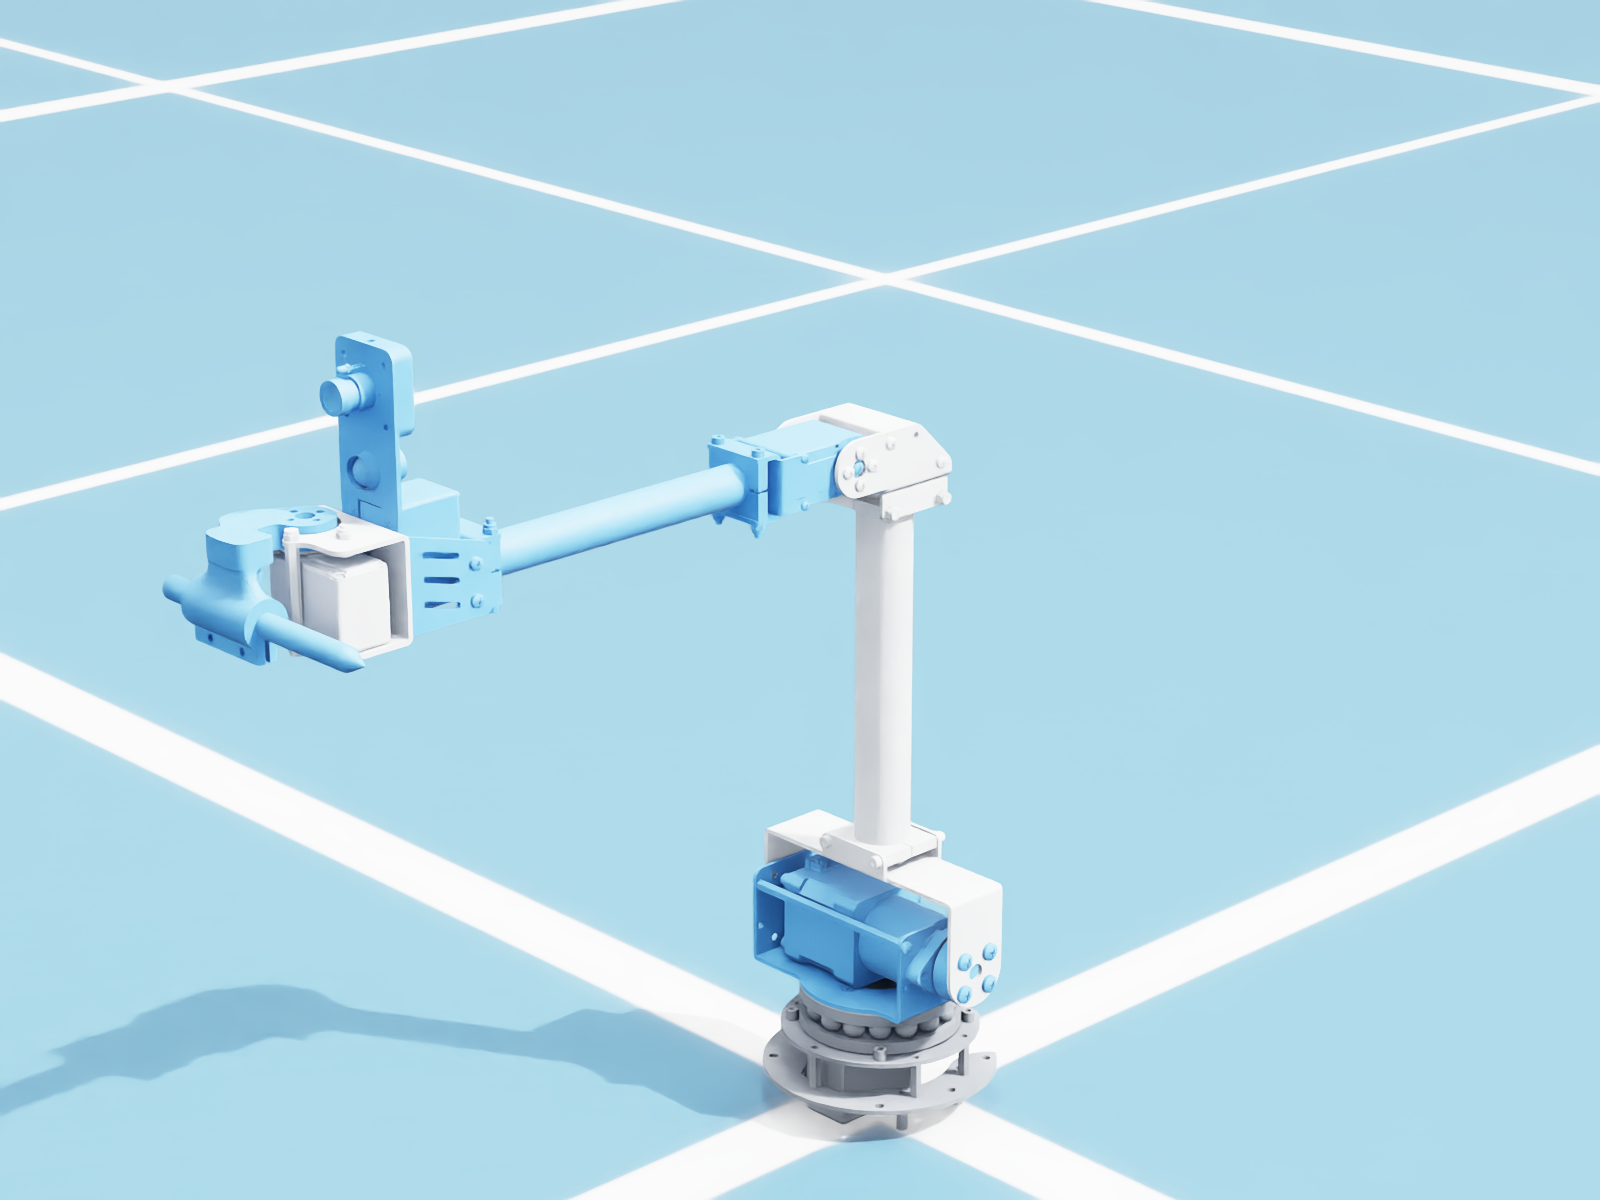
\includegraphics[width=0.72\textwidth]{zero_pose.png}
  \caption{Zero pose of the robotic arm}
  \label{fig:zero_pose}
\end{figure}

\begin{figure}[H]
  \centering
  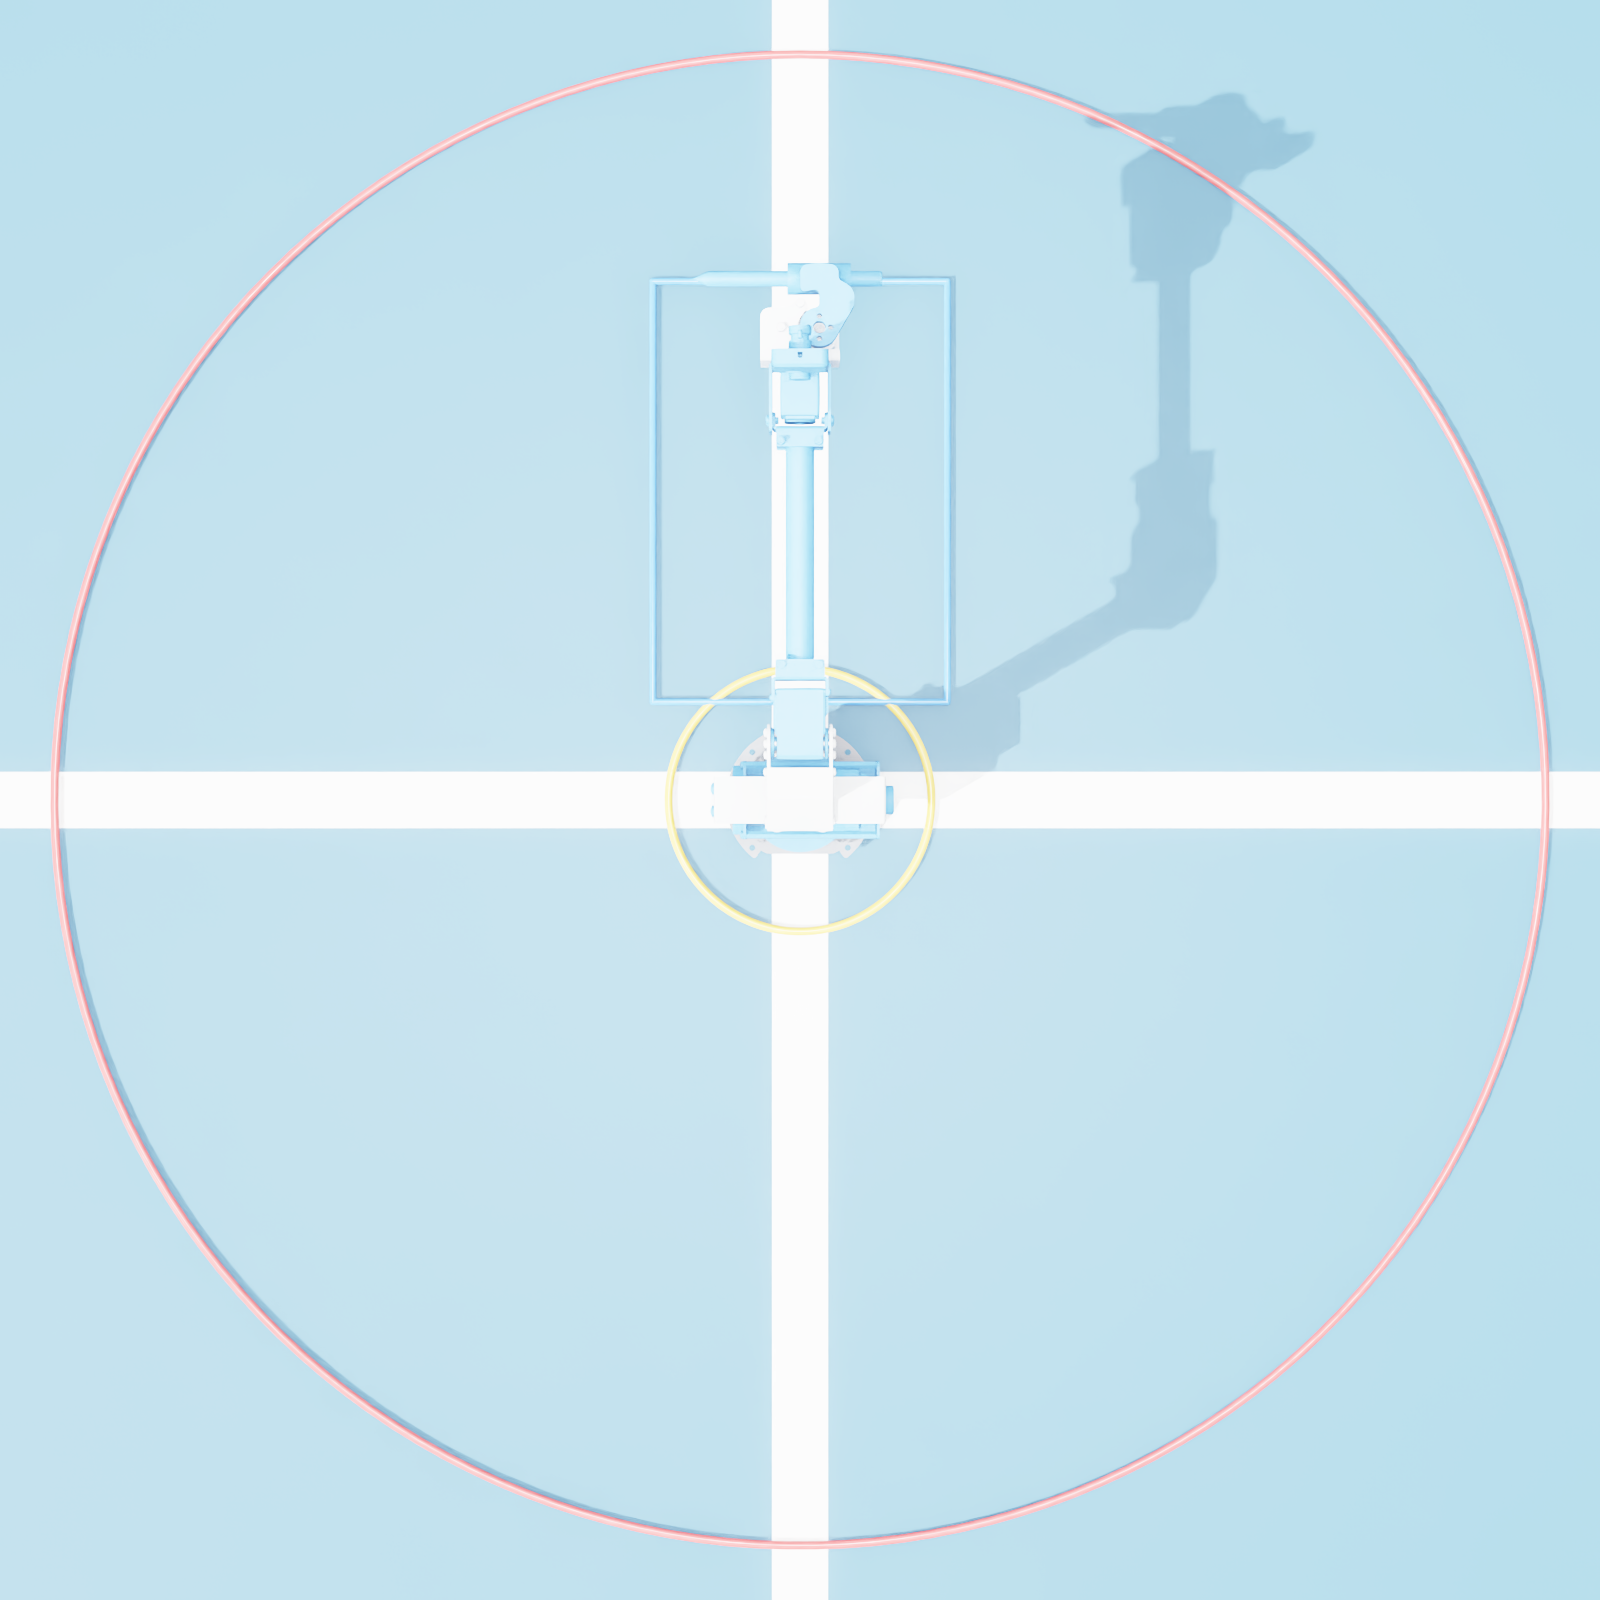
\includegraphics[width=0.72\textwidth]{reachable_area.png}
  \caption{Reachable workspace of the robotic arm}
  \label{fig:reachable}
\end{figure}

\subsection{Software Platform}

The project is implemented mainly in Python. OpenCV is used for paper detection, perspective transformation, binarization, and colored marker detection. NumPy and SciPy are used for coordinate mapping, trajectory resampling, and inverse-kinematics optimization. Isaac Sim is used for simulation and video rendering. The real-arm control link is implemented with Python sockets and pyserial.

\section{Overall System Design}

The end-to-end workflow is shown in Figure \ref{fig:pipeline}.

\begin{figure}[H]
  \centering
  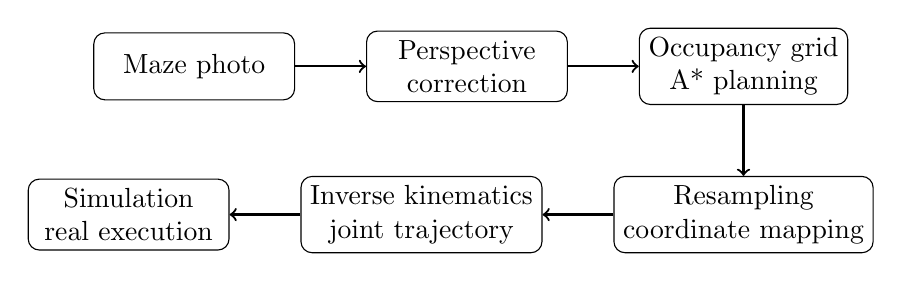
\begin{tikzpicture}[
    node distance=0.9cm and 0.9cm,
    box/.style={draw, rounded corners, align=center, minimum height=0.85cm, minimum width=2.55cm},
    arrow/.style={->, thick}
  ]
    \node[box] (a) {Maze photo};
    \node[box, right=of a] (b) {Perspective\\correction};
    \node[box, right=of b] (c) {Occupancy grid\\A* planning};
    \node[box, below=of c] (d) {Resampling\\coordinate mapping};
    \node[box, left=of d] (e) {Inverse kinematics\\joint trajectory};
    \node[box, left=of e] (f) {Simulation\\real execution};
    \draw[arrow] (a) -- (b);
    \draw[arrow] (b) -- (c);
    \draw[arrow] (c) -- (d);
    \draw[arrow] (d) -- (e);
    \draw[arrow] (e) -- (f);
  \end{tikzpicture}
  \caption{Overall system pipeline}
  \label{fig:pipeline}
\end{figure}

The vision and planning modules generate a pixel-space path. Both the simulation and real-arm client reuse the same pixel-to-world mapping and the same kinematics implementation in \texttt{arm\_kinematics.py}. This keeps the simulated and real trajectories consistent.

\section{Project Structure and Module Relationship}

The repository follows the robotics pipeline of perception, planning, kinematics, simulation, and real hardware control.

\begin{lstlisting}[language=bash, caption={Main project structure}]
Maze/
  maze_planner/          # Maze reconstruction and path planning
    maze_scanner.py      # Paper detection, perspective correction, binarization
    maze_planner.py      # Marker detection, occupancy grid, A* search
    samples/             # Test maze images
    outputs/             # Intermediate images and trajectory output

  arm_sim/               # Isaac Sim simulation and kinematic validation
    arm_kinematics.py    # 5-DOF forward and inverse kinematics
    draw_maze.py         # Simulated maze drawing
    draw_circle.py       # FK/IK validation by drawing a circle
    video/               # Rendered simulation videos

  arm_real_client/       # Upper-level client
    draw_maze_real.py    # Image -> path -> IK -> TCP trajectory command
    robot_client.py      # TCP JSON client wrapper
    estop.py             # Software stop command

  arm_real_server/       # Lower-level server
    robot_server.py      # TCP server, limits, point execution, feedback
    robot_server_openloop.py # Open-loop timed execution version

  urdf/                  # Robot model
    five_dof_arm.urdf
    meshes/

  assets/                # Demonstration images and simulation captures
\end{lstlisting}

The module relationship is shown in Figure \ref{fig:module_relation}. The planner produces a pixel path; the kinematics module converts it into joint angles; the simulation and real client consume the same joint trajectory.

\begin{figure}[H]
  \centering
  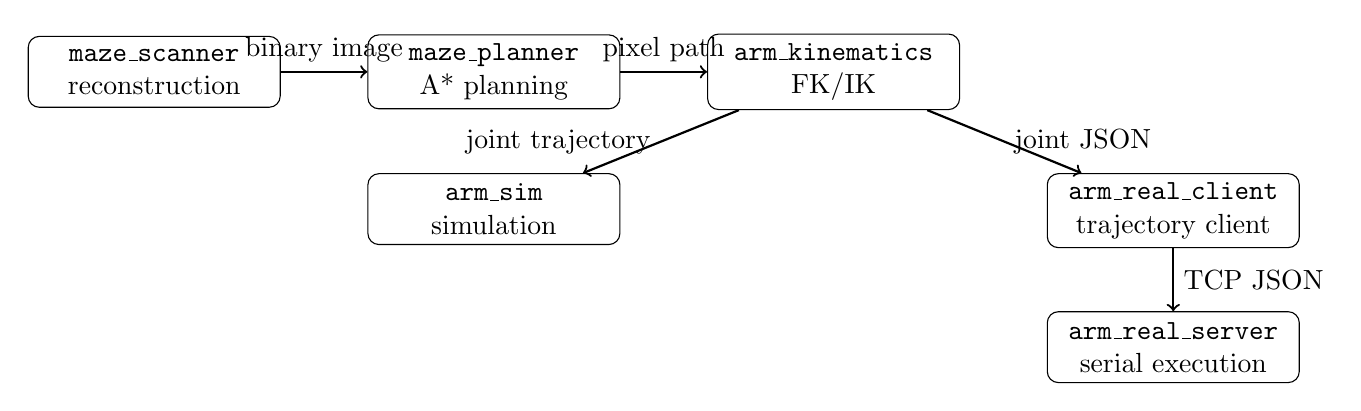
\begin{tikzpicture}[
    node distance=0.8cm and 1.1cm,
    box/.style={draw, rounded corners, align=center, minimum height=0.9cm, minimum width=3.2cm},
    arrow/.style={->, thick}
  ]
    \node[box] (scanner) {\texttt{maze\_scanner}\\reconstruction};
    \node[box, right=of scanner] (planner) {\texttt{maze\_planner}\\A* planning};
    \node[box, right=of planner] (kin) {\texttt{arm\_kinematics}\\FK/IK};
    \node[box, below left=of kin] (sim) {\texttt{arm\_sim}\\simulation};
    \node[box, below right=of kin] (client) {\texttt{arm\_real\_client}\\trajectory client};
    \node[box, below=of client] (server) {\texttt{arm\_real\_server}\\serial execution};
    \draw[arrow] (scanner) -- node[above]{binary image} (planner);
    \draw[arrow] (planner) -- node[above]{pixel path} (kin);
    \draw[arrow] (kin) -- node[left]{joint trajectory} (sim);
    \draw[arrow] (kin) -- node[right]{joint JSON} (client);
    \draw[arrow] (client) -- node[right]{TCP JSON} (server);
  \end{tikzpicture}
  \caption{Module relationship}
  \label{fig:module_relation}
\end{figure}

\section{Maze Image Reconstruction}

\subsection{Paper Detection and Perspective Correction}

The input photo may be tilted and affected by perspective distortion. The scanner first detects the paper region using brightness and saturation cues; if this fails, it falls back to edge-based detection. The four paper corners are ordered as top-left, top-right, bottom-right, and bottom-left, then a perspective transform is applied.

\begin{lstlisting}[language=Python, caption={Four-point perspective transformation}]
def four_point_transform(img, rect):
    tl, tr, br, bl = rect
    width_top = np.linalg.norm(tr - tl)
    width_bottom = np.linalg.norm(br - bl)
    height_left = np.linalg.norm(bl - tl)
    height_right = np.linalg.norm(br - tr)
    max_w = int(round(max(width_top, width_bottom)))
    max_h = int(round(max(height_left, height_right)))

    dst = np.array([[0, 0],
                    [max_w - 1, 0],
                    [max_w - 1, max_h - 1],
                    [0, max_h - 1]], dtype="float32")
    M = cv2.getPerspectiveTransform(rect, dst)
    return cv2.warpPerspective(img, M, (max_w, max_h))
\end{lstlisting}

\begin{figure}[H]
  \centering
  
\includegraphics[width=0.72\textwidth]{1_paper_detected.png}
  \caption{Detected paper contour}
\end{figure}

\begin{figure}[H]
  \centering
  
\includegraphics[width=0.72\textwidth]{2_warped.png}
  \caption{Perspective-corrected maze image}
\end{figure}

\subsection{Illumination Enhancement and Binarization}

Uneven lighting is handled by estimating a smooth background with a large Gaussian blur and normalizing the original grayscale image by this background. CLAHE is then applied to enhance local contrast, followed by adaptive thresholding.

\begin{lstlisting}[language=Python, caption={Illumination enhancement}]
def enhance(img):
    gray = cv2.cvtColor(img, cv2.COLOR_BGR2GRAY) if img.ndim == 3 else img
    k = max(31, (max(gray.shape) // 20) | 1)
    background = cv2.GaussianBlur(gray, (k, k), 0)
    background = np.where(background == 0, 1, background)
    norm = gray.astype(np.float32) / background.astype(np.float32)
    norm = np.clip(norm, 0, 1)
    norm = (norm * 255).astype(np.uint8)
    clahe = cv2.createCLAHE(clipLimit=2.0, tileGridSize=(8, 8))
    return clahe.apply(norm)
\end{lstlisting}

\begin{figure}[H]
  \centering
  \begin{subfigure}{0.48\textwidth}
    \centering
    
\includegraphics[width=\textwidth]{3_enhanced.png}
    \caption{Enhanced image}
  \end{subfigure}
  \hfill
  \begin{subfigure}{0.48\textwidth}
    \centering
    
\includegraphics[width=\textwidth]{4_binary.png}
    \caption{Binary image}
  \end{subfigure}
  \caption{Enhancement and binarization results}
\end{figure}

\begin{figure}[H]
  \centering
  
\includegraphics[width=0.72\textwidth]{5_result.png}
  \caption{Cleaned binary scan}
\end{figure}

\section{Path Planning}

\subsection{Mathematical Formulation}

Let the rectified binary image have size $W \times H$, and let a pixel be
\[
  p=(x,y), \quad 0 \le x < W,\ 0 \le y < H .
\]
The binary occupancy function is defined as
\[
  O(x,y)=
  \begin{cases}
    1, & I(x,y)<128,\ \text{wall or obstacle},\\
    0, & I(x,y)\ge 128,\ \text{free space}.
  \end{cases}
\]
The map is downsampled to a grid with maximum side length \texttt{grid\_max}. With scale
\[
  s=\frac{\texttt{grid\_max}}{\max(W,H)},
\]
the pixel coordinate is mapped to grid coordinate
\[
  c=(r,c)=\left(\left\lfloor sy \right\rceil,\left\lfloor sx \right\rceil\right).
\]
The planning graph is
\[
  G=(V,E), \qquad V=\{(r,c)\mid O_g(r,c)=0\},
\]
where $O_g$ is the processed occupancy grid. The objective is
\[
  P^*=\arg\min_P \sum_{i=1}^{n-1} w(c_i,c_{i+1}),
  \quad c_1=c_s,\ c_n=c_g .
\]

\subsection{Start and Goal Detection}

The start point is marked in red and the goal point is marked in blue. The planner converts the image to HSV space, thresholds red and blue masks, and uses the largest connected component centroid as the marker location.

\begin{lstlisting}[language=Python, caption={Red/blue marker detection}]
def detect_markers(bgr):
    hsv = cv2.cvtColor(bgr, cv2.COLOR_BGR2HSV)
    k = np.ones((5, 5), np.uint8)

    red = cv2.inRange(hsv, (0, 80, 40), (10, 255, 255)) | \
          cv2.inRange(hsv, (170, 80, 40), (180, 255, 255))
    red = cv2.morphologyEx(red, cv2.MORPH_OPEN, k)

    blue = cv2.inRange(hsv, (100, 80, 40), (130, 255, 255))
    blue = cv2.morphologyEx(blue, cv2.MORPH_OPEN, k)
    return _largest_blob_centroid(red), _largest_blob_centroid(blue)
\end{lstlisting}

\subsection{Occupancy Grid Construction}

The wall pixels are processed with marker erasing, morphological closing, conservative downsampling, and obstacle inflation. Obstacle inflation is equivalent to planning in configuration space:
\[
  \mathcal{O}_{\mathrm{inflated}}=\mathcal{O}\oplus B_{\rho},
\]
where $\oplus$ denotes the Minkowski sum and $B_{\rho}$ is the structuring element with radius $\rho$.

\begin{lstlisting}[language=Python, caption={Occupancy grid construction}]
def build_occupancy(binary, markers, close=5, inflate=1, grid_max=400):
    h0, w0 = binary.shape
    wall = (binary < 128).astype(np.uint8)

    erase_r = max(12, int(0.02 * max(h0, w0)))
    for m in markers:
        if m is not None:
            cv2.circle(wall, (int(round(m[0])), int(round(m[1]))),
                       erase_r, 0, -1)

    if close > 0:
        wall = cv2.morphologyEx(wall, cv2.MORPH_CLOSE,
                                np.ones((close, close), np.uint8))
    scale = grid_max / float(max(h0, w0))
    if scale < 1.0:
        gh, gw = max(int(h0 * scale), 1), max(int(w0 * scale), 1)
        wall = (cv2.resize(wall * 255, (gw, gh),
                           interpolation=cv2.INTER_AREA) > 0).astype(np.uint8)
    else:
        scale = 1.0
    if inflate > 0:
        wall = cv2.dilate(wall, np.ones((2 * inflate + 1,) * 2, np.uint8))
    return wall.astype(bool), scale
\end{lstlisting}

\begin{figure}[H]
  \centering
  
\includegraphics[width=0.72\textwidth]{6_occupancy.png}
  \caption{Occupancy grid: white is free space and black is obstacle}
\end{figure}

\subsection{A* Search}

The planner uses an 8-connected A* search. The evaluation function is
\[
  f(n)=g(n)+h(n),
\]
where $g(n)$ is the accumulated path cost and $h(n)$ is the Euclidean heuristic:
\[
  h(n)=\sqrt{(r_n-r_g)^2+(c_n-c_g)^2}.
\]
The Euclidean heuristic is admissible for the 8-connected grid, so A* returns an optimal discrete path. Diagonal moves are additionally checked to prevent cutting through a corner between two walls.

\begin{lstlisting}[language=Python, caption={A* neighbor expansion and diagonal check}]
for dr, dc, cost in nbrs:
    nr, nc = cr + dr, cc + dc
    if not (0 <= nr < h and 0 <= nc < w) or occ[nr, nc]:
        continue
    if dr != 0 and dc != 0 and (occ[cr + dr, cc] and occ[cr, cc + dc]):
        continue
    ng = g + cost
    if ng < gscore.get((nr, nc), float("inf")):
        gscore[(nr, nc)] = ng
        came[(nr, nc)] = cur
        heapq.heappush(open_heap, (ng + heur((nr, nc), goal), ng, (nr, nc)))
\end{lstlisting}

\begin{figure}[H]
  \centering
  
\includegraphics[width=0.75\textwidth]{planned.png}
  \caption{Planned maze path}
\end{figure}

\section{Kinematics and Trajectory Generation}

\subsection{Pixel-to-Paper Coordinate Mapping}

For a rectified image point $(p_x,p_y)$ with image size $(W,H)$, the normalized coordinates are
\[
  u=\frac{p_x}{W}, \qquad v=\frac{p_y}{H}.
\]
Let the paper size be $L_x=0.30\ \mathrm{m}$ and $L_y=0.21\ \mathrm{m}$, and let the paper center be $(x_c,y_c,z_{\mathrm{paper}})$. The target pen-tip point is
\[
  \mathbf{x}_d =
  \begin{bmatrix}
    x_c + (0.5-v)L_x \\
    y_c + (u-0.5)L_y \\
    z_{\mathrm{paper}}+\Delta z
  \end{bmatrix},
\]
where $\Delta z=0.001\ \mathrm{m}$.

\begin{lstlisting}[language=Python, caption={Image coordinate to paper coordinate mapping}]
PAPER_SX, PAPER_SY, PAPER_TOP = 0.30, 0.21, 0.002
PEN_Z = PAPER_TOP + 0.001

def img_to_world(px, py, wimg, himg, paper_cx, paper_cy):
    u, v = px / wimg, py / himg
    return (paper_cx + (0.5 - v) * PAPER_SX,
            paper_cy + (u - 0.5) * PAPER_SY, PEN_Z)
\end{lstlisting}

\subsection{Arc-Length Resampling}

The A* output is a grid polyline. To make the robot trajectory more uniform, the path is resampled by arc length. Given
\[
  P=\{\mathbf{p}_0,\mathbf{p}_1,\ldots,\mathbf{p}_{m-1}\},
\]
the cumulative length is
\[
  l_0=0,\qquad
  l_i=\sum_{k=1}^{i}\|\mathbf{p}_k-\mathbf{p}_{k-1}\|_2 .
\]
For $N$ waypoints,
\[
  \hat{l}_j=\frac{j}{N-1}l_{m-1}, \qquad j=0,1,\ldots,N-1 .
\]

\begin{lstlisting}[language=Python, caption={Arc-length resampling}]
def resample(pts, n):
    P = np.asarray(pts, float)
    d = np.r_[0, np.cumsum(np.linalg.norm(np.diff(P, axis=0), axis=1))]
    s = np.linspace(0, d[-1], n)
    return np.c_[np.interp(s, d, P[:, 0]), np.interp(s, d, P[:, 1])]
\end{lstlisting}

\subsection{Forward Kinematics}

Let the joint vector be
\[
  \mathbf{q}=[q_1,q_2,q_3,q_4,q_5]^T .
\]
Each joint transform is modeled from the URDF fixed origin and the joint-axis rotation:
\[
  {}^{i-1}T_i(q_i)=
  \begin{bmatrix}
    R_i^{0}R_z(\sigma_i q_i) & \mathbf{t}_i\\
    \mathbf{0}^T & 1
  \end{bmatrix}.
\]
The end-effector transform is
\[
  {}^{0}T_5(\mathbf{q})=\prod_{i=1}^{5}{}^{i-1}T_i(q_i).
\]
If the pen tip in the link-5 frame is ${}^{5}\mathbf{p}_{nib}$, then
\[
  {}^{0}\mathbf{p}_{nib}
  ={}^{0}R_5(\mathbf{q})\,{}^{5}\mathbf{p}_{nib}
  +{}^{0}\mathbf{t}_5(\mathbf{q}).
\]

\begin{lstlisting}[language=Python, caption={Forward kinematics}]
def fk_M5(q):
    M = np.eye(4)
    for (tr, rot, sign), th in zip(_JOINTS, q):
        M = M @ tr @ rot @ _Rz(sign * th)
    return M

def fk_nib_tail(q):
    M5 = fk_M5(q)
    o, R = M5[:3, 3], M5[:3, :3]
    return o + R @ _NIB, o + R @ _TAIL
\end{lstlisting}

Although a pen-tip Jacobian can be defined as
\[
  J_p(\mathbf{q})=
  \frac{\partial\,{}^{0}\mathbf{p}_{nib}}{\partial \mathbf{q}}
  \in\mathbb{R}^{3\times 5},
\]
the current branch does not explicitly construct this Jacobian. Instead, the forward-kinematics function is directly passed to the SLSQP nonlinear optimizer.

\subsection{Inverse Kinematics}

The IK solver uses bounded SLSQP optimization. The first stage minimizes position error:
\[
  \mathbf{q}_{pos}=
  \arg\min_{\mathbf{q}_{min}\le\mathbf{q}\le\mathbf{q}_{max}}
  \|\mathbf{p}_{nib}(\mathbf{q})-\mathbf{x}_d\|_2^2 .
\]
If the target is reachable, the second stage keeps the pen tip fixed and optimizes the pen axis. Let
\[
  \mathbf{a}(\mathbf{q})=
  \frac{\mathbf{p}_{nib}(\mathbf{q})-\mathbf{p}_{tail}(\mathbf{q})}
       {\|\mathbf{p}_{nib}(\mathbf{q})-\mathbf{p}_{tail}(\mathbf{q})\|_2}.
\]
The desired axis is downward, $\mathbf{a}_d=[0,0,-1]^T$, and the orientation objective is
\[
  \mathbf{q}^{*}=
  \arg\min_{\mathbf{q}_{min}\le\mathbf{q}\le\mathbf{q}_{max}}
  (1+a_z(\mathbf{q}))
  +\lambda\|\mathbf{q}-\mathbf{q}_{ref}\|_2^2,
\]
\[
  \mathrm{s.t.}\quad
  \mathbf{p}_{nib}(\mathbf{q})=\mathbf{x}_d .
\]

\begin{lstlisting}[language=Python, caption={Inverse kinematics framework}]
def ik(target, q0, lim=None):
    del lim
    target = np.asarray(target, float)
    q_ref = np.clip(np.asarray(q0, float), _JOINT_LO, _JOINT_HI)

    def pos_cost(q):
        err = fk_pos(q) - target
        return float(err @ err)

    pos_res = minimize(pos_cost, q_ref, method="SLSQP", bounds=_BOUNDS)
    q_pos = np.clip(pos_res.x if pos_res.x is not None else q_ref,
                    _JOINT_LO, _JOINT_HI)
    pos_err = float(np.linalg.norm(fk_pos(q_pos) - target))

    if pos_err > _POS_TOL:
        a = _pen_axis(q_pos)
        tilt = np.degrees(np.arccos(np.clip(-a[2], -1, 1)))
        return q_pos, pos_err, float(tilt)

    def orient_cost(q):
        a = _pen_axis(q)
        return float((1.0 + a[2]) + _CONTINUITY_W * np.sum((q - q_ref) ** 2))

    orient_res = minimize(orient_cost, q_pos, method="SLSQP",
                          bounds=_BOUNDS,
                          constraints=({"type": "eq",
                                        "fun": lambda q: fk_pos(q) - target},))
    q = np.clip(orient_res.x if orient_res.x is not None else q_pos,
                _JOINT_LO, _JOINT_HI)
    if np.linalg.norm(fk_pos(q) - target) > max(_POS_TOL, pos_err * 2.0):
        q = q_pos
    a = _pen_axis(q)
    tilt = np.degrees(np.arccos(np.clip(-a[2], -1, 1)))
    return q, float(np.linalg.norm(fk_pos(q) - target)), float(tilt)
\end{lstlisting}

The current joint limits are
\[
  \mathbf{q}_{min}=[-180,-90,-90,-90,-45]^\circ,\quad
  \mathbf{q}_{max}=[180,90,90,90,45]^\circ .
\]
The fifth joint $h$ is now used as a pen-rotation joint, but the real usable range is still treated as $\pm45^\circ$.

The current trajectory file contains 70 points. Its metadata is summarized in Table \ref{tab:traj_meta}.

\begin{table}[H]
  \centering
  \caption{Trajectory metadata}
  \label{tab:traj_meta}
  \begin{tabular}{ll}
    \toprule
    Item & Value \\
    \midrule
    Source image & \texttt{maze\_planner/samples/test\_0.jpg} \\
    Number of waypoints & 70 \\
    Paper center distance & \texttt{paper\_cx = 0.22 m} \\
    Time interval & \texttt{dt = 0.1 s} \\
    Maximum IK residual & about $0.0494$ mm \\
    Maximum pen-axis tilt & about $0.572^\circ$ \\
    \bottomrule
  \end{tabular}
\end{table}

\section{Isaac Sim Verification}

The simulation module imports the URDF into Isaac Sim and maps the reconstructed maze as a texture on a $30\ \mathrm{cm} \times 21\ \mathrm{cm}$ paper plane. The robot joint positions are set point by point, and a red trail visualizes the drawn path.

\begin{lstlisting}[language=Python, caption={Simulation trajectory generation}]
pts, warped, binary, start_xy, goal_xy = solve_path(MAZE_IMG, auto=True,
                                                    debug_dir=_IMG_DIR)
path_px = resample(pts, N_WAYPOINTS)
targets = [img_to_world(px, py, wimg, himg) for px, py in path_px]

qtraj, res, tilt = [], [], []
q_seed = np.array([0.0, 1.0, 1.0, 0.0, 0.0])
for tgt in targets:
    q_seed, e, ti = ik(np.array(tgt), q_seed)
    qtraj.append(q_seed.copy())
    res.append(e)
    tilt.append(ti)
\end{lstlisting}

Simulation videos are stored in \texttt{arm\_sim/video/}, including joint-motion demonstration, circle drawing, and maze drawing.

\maybeimage{Key frame of Isaac Sim maze drawing}{figures/sim_draw_maze_frame.jpg}

\section{Real Robotic Arm Control}

\subsection{Communication Architecture}

The real system follows an upper/lower-level architecture. The upper-level client performs planning and IK, while the lower-level Windows server communicates with the robot over serial and exposes a TCP JSON API.

\begin{figure}[H]
  \centering
  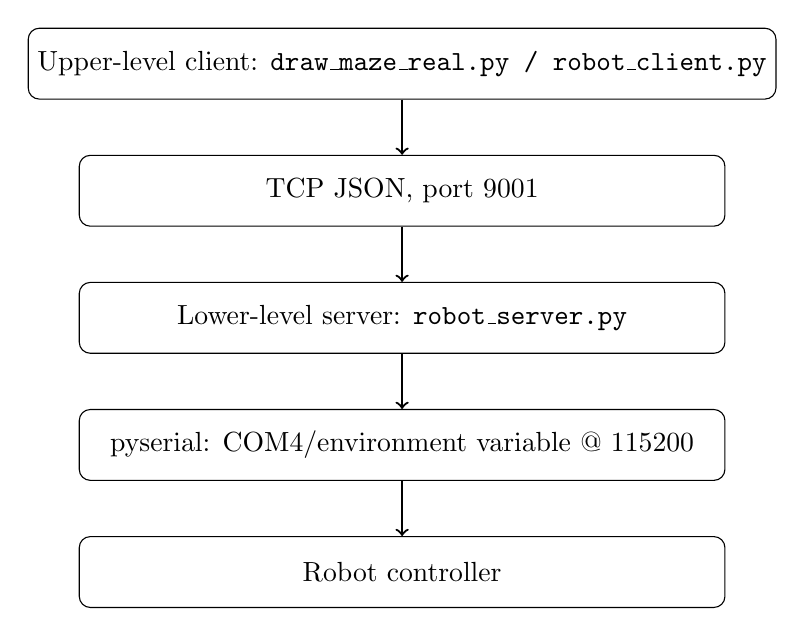
\begin{tikzpicture}[
    node distance=0.7cm,
    box/.style={draw, rounded corners, align=center, minimum height=0.9cm, minimum width=8.2cm},
    arrow/.style={->, thick}
  ]
    \node[box] (a) {Upper-level client: \texttt{draw\_maze\_real.py / robot\_client.py}};
    \node[box, below=of a] (b) {TCP JSON, port 9001};
    \node[box, below=of b] (c) {Lower-level server: \texttt{robot\_server.py}};
    \node[box, below=of c] (d) {pyserial: COM4/environment variable @ 115200};
    \node[box, below=of d] (e) {Robot controller};
    \draw[arrow] (a) -- (b);
    \draw[arrow] (b) -- (c);
    \draw[arrow] (c) -- (d);
    \draw[arrow] (d) -- (e);
  \end{tikzpicture}
  \caption{Real-arm communication chain}
\end{figure}

The current server listens on \texttt{0.0.0.0:9001} by default. The serial port defaults to \texttt{COM4} on Windows and can be overridden with \texttt{ROBOT\_SERIAL\_PORT}. The host and port can also be overridden with \texttt{ROBOT\_SERVER\_HOST} and \texttt{ROBOT\_SERVER\_PORT}.

\subsection{TCP Client}

\begin{lstlisting}[language=Python, caption={Trajectory request in the upper-level client}]
class RobotClient:
    def request(self, payload):
        msg = json.dumps(payload, separators=(",", ":")) + "\n"
        with socket.create_connection((self.host, self.port),
                                      timeout=self.timeout) as sock:
            sock.sendall(msg.encode("utf-8"))
            data = sock.recv(4096)
        return json.loads(data.decode("utf-8"))

    def trajectory(self, points, dt=DEFAULT_DT, traj_id="traj",
                   spd=DEFAULT_SPD, acc=DEFAULT_ACC):
        return self.request({
            "type": "trajectory",
            "traj_id": traj_id,
            "dt": dt,
            "spd": spd,
            "acc": acc,
            "points": points,
        })
\end{lstlisting}

\subsection{Serial Command Generation}

The lower-level server converts joint targets into the arm's serial JSON protocol. Joint control uses command type \texttt{T=122}.

\begin{lstlisting}[language=Python, caption={Serial joint command generation}]
def make_arm_cmd(point, global_spd=None, global_acc=None):
    cmd = {"T": 122}
    for joint, (lo, hi) in LIMITS.items():
        value = point.get(joint, 0.0)
        cmd[joint] = clamp(value, lo, hi)
    cmd["spd"] = point.get("spd", global_spd if global_spd is not None else DEFAULT_SPD)
    cmd["acc"] = point.get("acc", global_acc if global_acc is not None else DEFAULT_ACC)
    return cmd
\end{lstlisting}

\begin{table}[H]
  \centering
  \caption{Server API}
  \begin{tabular}{ll}
    \toprule
    Request & Function \\
    \midrule
    \texttt{ping} & Connectivity test \\
    \texttt{joint} & Send a single joint target \\
    \texttt{trajectory} & Asynchronously execute a full trajectory \\
    \texttt{status} & Query local execution state \\
    \texttt{state} & Query low-level robot state \\
    \texttt{stop} & Stop sending subsequent trajectory points \\
    \bottomrule
  \end{tabular}
\end{table}

\subsection{Trajectory Execution Strategy}

When a trajectory is received, the server starts a worker thread. It first checks whether \texttt{T=1051} state feedback is available. If feedback works, it uses \texttt{poll-until-reached}: send one point, wait until the feedback angles stabilize, then send the next point. If feedback is unavailable, it falls back to \texttt{timed(dt)} mode and waits a fixed time after each command.

\subsection{Real-Arm Trajectory Preprocessing}

The current branch performs two additional preprocessing steps before sending the trajectory. First, backlash compensation can be applied through \texttt{--backlash-s-deg} and \texttt{--backlash-e-deg}. Shoulder compensation is triggered according to the direction of $|s|$, while elbow compensation is triggered according to the raw direction of $e$.

\begin{lstlisting}[language=Python, caption={Backlash compensation entry point}]
def apply_backlash_compensation(points, s_deg, e_deg):
    n_s = _apply_shoulder_backlash(points, s_deg)
    n_e = _apply_directional_backlash(points, "e", e_deg)
    if n_s or n_e:
        print(f"[backlash] s={s_deg:+.2f}, e={e_deg:+.2f}", flush=True)
\end{lstlisting}

Second, a pre-turn point is inserted before the actual path. This point uses the first path point's \texttt{b/s/e/w} values but keeps \texttt{h=0}, reducing sudden end-effector posture changes at the beginning of drawing.

\begin{lstlisting}[language=Python, caption={Prepending an h=0 pre-turn point}]
def prepend_w_preturn_point(points):
    pre = dict(points[0])
    pre["h"] = 0.0
    return [pre] + points
\end{lstlisting}

\maybeimage{Real arm at the beginning of drawing}{figures/real_drawing_start.jpg}
\maybeimage{Final real-arm drawing result}{figures/real_result.jpg}

\section{Experimental Procedure}

\subsection{Maze Planning}

\begin{lstlisting}[language=bash, caption={Maze reconstruction and planning}]
conda env create -f maze_planner/environment.yml
conda activate maze
python maze_planner/maze_planner.py maze_planner/samples/test_0.jpg \
  -o maze_planner/outputs/image/planned.png --auto
\end{lstlisting}

\subsection{Simulation}

\begin{lstlisting}[language=bash, caption={Isaac Sim command}]
python arm_sim/draw_maze.py
\end{lstlisting}

\subsection{Real-Arm Dry Run}

\begin{lstlisting}[language=bash, caption={Trajectory generation and dry-run check}]
python arm_real_client/draw_maze_real.py --n-waypoints 70
\end{lstlisting}

The default mode plans, solves IK, checks limits, and saves the trajectory without connecting to hardware. The trajectory is written to \texttt{maze\_planner/outputs/trajectory/trajectory.json}. Backlash compensation can be added with \texttt{--backlash-s-deg} and \texttt{--backlash-e-deg}.

\subsection{Real-Arm Execution}

\begin{lstlisting}[language=bash, caption={First hardware test with a few points}]
python arm_real_client/draw_maze_real.py --send --from-file --max-points 5
\end{lstlisting}

\begin{lstlisting}[language=bash, caption={Full hardware execution}]
python arm_real_client/draw_maze_real.py --send --from-file
\end{lstlisting}

\begin{lstlisting}[language=bash, caption={Software stop}]
python arm_real_client/estop.py
\end{lstlisting}

\section{Results and Analysis}

\subsection{Image Processing Result}

The reconstruction pipeline successfully detects the paper region, corrects perspective distortion, and produces a clean binary image suitable for path planning.

\begin{figure}[H]
  \centering
  
\includegraphics[width=0.72\textwidth]{0_input.png}
  \caption{Original input photo}
\end{figure}

\begin{figure}[H]
  \centering
  
\includegraphics[width=0.72\textwidth]{planned.png}
  \caption{Final planned path}
\end{figure}

\subsection{Path Planning Result}

The planned path connects the red start marker to the blue goal marker while avoiding inflated wall regions. The diagonal corner check prevents the algorithm from exploiting unrealistic one-pixel corner gaps.

\subsection{Kinematic Result}

The current trajectory file reports a maximum IK position residual of approximately $0.0494\ \mathrm{mm}$ and a maximum pen-axis tilt of approximately $0.572^\circ$. This indicates that the robot model can reach the full maze path with a nearly vertical pen posture under the current paper placement. Before real execution, joint-limit checking is still necessary; if any angle exceeds the real soft limits, the lower-level server clamps the command, which may distort the final drawing.

\subsection{Real Hardware Result}

The repository does not yet include real hardware photos. After adding them, the result should be evaluated by start-point accuracy, global path offset, corner quality, wall collision, and final goal error.

\maybeimage{Comparison between real drawing and planned path}{figures/real_vs_plan.jpg}

\section{Issues and Future Work}

First, the paper pose is still manually configured by \texttt{paper\_cx} and \texttt{paper\_cy}. Future work can introduce ArUco markers or camera-to-robot calibration.

Second, the real trajectory is executed point by point. This is stable but slow. Continuous trajectory interpolation or velocity planning could make the drawing smoother.

Third, pen pressure is not closed-loop controlled in this branch. A future version could use torque feedback or an external pressure sensor for adaptive $z$-axis regulation.

Fourth, the pen posture is limited by the robot's joint range, especially the real $\pm45^\circ$ limit of joint $h$ and the conservative $\pm90^\circ$ limit of joint $w$.

Fifth, the vision pipeline still depends on lighting and background conditions. More robust segmentation or fiducial markers could improve reliability.

\section{Conclusion}

This experiment implements a complete robotic maze drawing system from vision input to real-arm execution. The system reconstructs a paper maze from a camera photo, plans a path using an occupancy-grid A* algorithm, maps the 2-D path to physical paper coordinates, solves bounded inverse kinematics for a 5-DOF robotic arm, verifies the motion in Isaac Sim, and sends the resulting joint trajectory to real hardware through a TCP and serial communication chain.

\appendix
\section{Key Files}

\begin{longtable}{p{6cm}p{8cm}}
  \caption{Key project files} \\
  \toprule
  File & Role \\
  \midrule
  \endfirsthead
  \toprule
  File & Role \\
  \midrule
  \endhead
  \texttt{maze\_planner/maze\_scanner.py} & Paper detection, perspective correction, enhancement, and binarization \\
  \texttt{maze\_planner/maze\_planner.py} & Marker detection, occupancy-grid construction, and A* planning \\
  \texttt{arm\_sim/arm\_kinematics.py} & Forward and inverse kinematics for the 5-DOF arm \\
  \texttt{arm\_sim/draw\_maze.py} & Isaac Sim rendering of maze drawing \\
  \texttt{arm\_real\_client/draw\_maze\_real.py} & Converts the maze path to a real-arm joint trajectory \\
  \texttt{arm\_real\_client/robot\_client.py} & TCP client wrapper \\
  \texttt{arm\_real\_server/robot\_server.py} & TCP server and serial command execution \\
  \texttt{maze\_planner/outputs/image/} & Intermediate images and planning visualization \\
  \texttt{maze\_planner/outputs/trajectory/trajectory.json} & Executable joint trajectory \\
  \bottomrule
\end{longtable}

\end{document}
